\chapter{Riemann Surfaces}
\begin{chout}
	We now define Riemann surfaces, considering initial examples.
\end{chout}

\section{Definition}
\begin{definition}[Riemann surface]
	A \defined{Riemann surface} is a connected, one-dimensional complex analytic
	manifold.
\end{definition}

\begin{remark}
	Since we made the inclusion of second countability in our definition of a
	topological manifold, it is important to make comment on the fact that this
	inclusion is redundant for Riemann surfaces. In particular, every connected
	Riemann Surface is second countable; a highly non-trivial result due to Tibor
	Rad\'o\sidenotemark.

	We also note that an assertion of connectedness is not universal in the
	literature, but for our considerations, it is convenient.
\end{remark}
\sidenotetext[][-4\baselineskip]{\footnotesize \cite{rado}}

The concision of this definition is maybe unexpected, and it is
common\sidenote{\footnotesize\cite[p. 29]{donaldson}} to define Riemann surfaces
with a more verbose definition without the abstraction to manifolds, although
our approach is equivalent. A keen eye will note that this definition also
determines that we have already encountered an example of a Riemann surface ---
the Riemann sphere $ \hat{\mathbb{C}} $, is one dimensional and a suitable atlas
was given in Example~\ref{ex:Ch-analytic-manifold}.

\begin{example}\label{ex:C-open-subset}
	With reference to Example~\ref{ex:C-top-manifold}, $ \mathbb{C} $ is a Riemann
	surface. We call this Riemann surface the \defined{complex plane}.
\end{example}

We now consider some further examples in full detail as these will be useful in
providing future examples as we develop the theory in parallel.

\section{Projective line}
\begin{definition}[Complex Projective Line]
	The \defined{complex projective line}, denoted $ \mathbb{C}\mathbb{P}^{1} $ is
	the set of one dimensional subspaces of $ \mathbb{C}^{2} $.
\end{definition}

\begin{marginfigure}[-3\baselineskip]
	\centering
	\includegraphics{real-projective/figure}
	\caption{It is useful to consider these notions via their real analogues.}
\end{marginfigure}

We know from linear algebra that one dimensional subspaces are spanned by a
single element. For an element $ (x,y) \in \mathbb{C}^{2}\setminus \left\{ 0
	\right\} $, we denote the span of $ (x,y) $ by,
\begin{align*}
	[x:y] = \left\{ \lambda(x,y): \lambda \in \mathbb{C} \right\}.
\end{align*}
Hence, an alternative expression of $ \mathbb{C}\mathbb{P}^{1} $ is given as,
\begin{align*}
	\mathbb{C}\mathbb{P}^{1} = \left\{ [x:y]:(x,y) \in \mathbb{C}^{2}\setminus
	\left\{ 0 \right\} \right\}.
\end{align*}
We refer to the elements $ [x:y] \in \mathbb{C}\mathbb{P}^{1} $ as
\defined{homogeneous coordinates} since $ \forall \lambda \in
	\mathbb{C}^{*} $,
\begin{align*}
	[x:y] = [\lambda x: \lambda y].
\end{align*}

We now aim to give topological structure to $ \mathbb{C}\mathbb{P}^{1} $, and
from this, Riemann surface structure. For this process, we take inspiration from
Miranda\sidenote{\footnotesize\cite[p. 8]{miranda}}.

Consider the following two subsets of $ \mathbb{C}\mathbb{P}^{1} $,
\begin{align*}
	U_x & = \left\{ [x:y] : x \neq 0 \right\}, \\
	U_y & = \left\{ [x:y] : y \neq 0 \right\},
\end{align*}
which are clearly such that $ \mathbb{C}\mathbb{P}^{1} = U_x \cup U_y $. We
consider the following functions on these subsets;
\begin{align*}
	\phi_x: U_x \to \mathbb{C}: [x:y] \mapsto \frac{y}{x}, \\
	\phi_y: U_y \to \mathbb{C}: [x:y] \mapsto \frac{x}{y}.
\end{align*}
It is clear that these functions are respectively bijective. With this we can
give each $ U_i $ a topology; a set $ U \subseteq U_i $ is open if and only if $
	\phi_i(U) $ is open in $ \mathbb{C} $. Since the subsets $ U_i $ cover $
	\mathbb{C}\mathbb{P}^{1} $ we can equally well give this space a topology,
asserting that $ U \subseteq \mathbb{C}\mathbb{P}^{1} $ is open if and only if $
	U \cap U_i $ is open for each $ i=x,y $.

This definitively determines that $ (U_x, \phi_x) $ and $ (U_y, \phi_y) $
are charts on $ \mathbb{C}\mathbb{P}^{1} $, and furthermore, these charts are
compatible, since
\begin{align*}
	\phi_x \circ \phi_y ^{-1}(z) = \frac{1}{z} = \phi_y \circ \phi_x ^{-1}(z)
\end{align*}
is holomorphic on $ \phi_x(U_x \cap U_y) = \mathbb{C}^{*} = \phi_y(U_x \cap U_y)
$.

It remains to show that $ \mathbb{C}\mathbb{P}^{1} $ is Hausdorff. As usual,
we consider two points $ p,q \in \mathbb{C}\mathbb{P}^{1} $. If these points are
simultaneously contained by either $ U_x $ or $ U_y $, they may be separated by
disjoint open sets since the $ U_i $ are individually Hausdorff. The remaining
case is that of the points $ p=[1:0] $ and $ q=[0:1] $. These points are
respectively contained by the disjoint sets $ \phi_x ^{-1}(D) $ and $ \phi_y
	^{-1}(D) $ where $ D \subseteq \mathbb{C} $ is the open unit
disc\sidenote{\footnotesize\cite[p. 9]{miranda}}.

\begin{remark}
	There is a remarkable similarity between the approach seen here and the one we
	took for the Riemann sphere, which is, as usual in mathematics, no
	coincidence. We can show that as topological spaces $ \hat{\mathbb{C}} $ and $
		\mathbb{C}\mathbb{P}^{1} $ are homeomorphic via the map
	\begin{align*}
		g: \hat{\mathbb{C}} \to \mathbb{C}\mathbb{P}^{1}:z \mapsto \begin{cases}
			                                                           [z:1] & z \neq \infty \\
			                                                           [1:0] & z = \infty
		                                                           \end{cases}
	\end{align*}
	which is continuous and has continuous inverse,
	\begin{align*}
		h: \mathbb{C}\mathbb{P}^{1} \to \hat{\mathbb{C}}: [x:y] \mapsto \begin{cases}
			                                                                \frac{x}{y} & y \neq0 \\
			                                                                \infty
			                                                                            & y = 0.
		                                                                \end{cases}
	\end{align*}
	Furthermore, we will see in Section~\ref{sec:riemann-roch} that there is only
	one possible holomorphic structure on $ \hat{\mathbb{C}} $, the same as the
	one we have given to $ \mathbb{C}\mathbb{P}^{1} $.
\end{remark}

\section{Complex Tori}\label{sec:complex-tori}
We now aim to give Riemann surface structure to complex tori. We will, in fact,
consider one specific torus, although the approach is easily generalisable.
Firstly, we recall the definition of the Gaussian integers,
\begin{align*}
	\mathbb{Z} \oplus i \mathbb{Z} = \left\{ a + ib: a,b \in \mathbb{Z} \right\}
\end{align*}
which we choose to refer to by $ \Lambda $.

\begin{marginfigure}
	\centering
	\includegraphics{lattice/figure}
	\caption{We refer to discrete additive subgroups like $ \Lambda $ as lattices.}
\end{marginfigure}

We can construct the quotient space $ \mathbb{C}/\Lambda $, which is more
explicitly expressed as,
\begin{gather*}
	\mathbb{C}/{\sim} = \left\{ [z]: z \in \mathbb{C} \right\},\\
	[z] = \left\{ \omega \in \mathbb{C}: z \sim \omega \right\},\\
	z\sim \omega \iff z-\omega \in \Lambda.
\end{gather*}

This space has a natural quotient topology via the projection map $
	\pi:\mathbb{C}\to \mathbb{C}/\Lambda: z \mapsto [z] $. Further to this, we can
show that $ \pi $ is open --- considering an open set $ U \subseteq \mathbb{C}
$, showing that $ \pi(U) $ is open is simply noticing that
\begin{align*}
	\pi ^{-1}(\pi(U)) = \bigcup_{\lambda \in \Lambda}^{}{(\lambda + U)}
\end{align*}
is a union of translations of $ U $ by elements in $ \Lambda $; hence open.

\begin{marginfigure}
	\centering
	\includegraphics{pi-open/figure}
	\caption{$ \lambda _{a,b} = U + a + ib $}
\end{marginfigure}

In order to find a covering set of charts, we consider sets of the form
\begin{align*}
	B(z_0;\epsilon) = \left\{ \omega \in \mathbb{C}: |z_0-z|<\epsilon \right\},
\end{align*}
and note that for $ 0<\epsilon<\frac{1}{2} $, the map $
	\pi|_{B(z_0;\epsilon)}:B(z_0;\epsilon) \to \pi(B(z_0;\epsilon))$ is injective.
Furthermore, as a restriction of $ \pi $, this map is continuous, surjective,
and open, and this is sufficient to state $ \pi|_{B(z_0;\epsilon)} $ as a
homeomorphism between these two sets. Setting $ \phi _{z_0} $ to be the inverse of
this homeomorphism gives us a complex chart at the point $ \pi(z_0) = [z_0] $.
This shows $ \mathbb{C}/\Lambda $ to be locally Euclidean, and the compatibility
of these charts is all that stands between the realisation of a Riemann surface
structure.

For brevity, let $ U _{\alpha} $ denote the domain of the coordinate $ \phi
	_{\alpha} $, that is, the set $ \pi(B(\alpha; \epsilon)) $. The transition
function $ \phi _{z, \omega}: \phi _{\omega}(U_z \cap U _{\omega}) \to \phi
	_{z}( U_z \cap U _{\omega}) $ is such that
\begin{align*}
	\pi(\phi _{z,\omega})(u) & = \pi( \phi_z \circ \phi_{\omega}^{-1})(u) \\
	                         & = \phi_{\omega}^{-1}(u)                    \\
	                         & = \pi(u)
\end{align*}
for every $ u \in \phi _{\omega}(U_z \cap U _{\omega}) $, and notably, this
determines that $ \phi _{\omega}(u) \sim u $. We now observe that $ \phi _{z,
		\omega} $ is continuous, and that $ \Lambda $ is discrete. $ \phi _{z,
		\omega}(u)-u $ is therefore constant on the connected components of $ \phi
	_{\omega}(U_z \cap U _{\omega}) $ and $ \phi _{z, \omega} $ is holomorphic. The
charts are compatible.

To justify our naming of the section as `Complex Tori' we claim that the above
constructed quotient space is homeomorphic to the torus, defined as $ S^1 \times
	S^1$ for $ S^1 = \left\{ z \in \mathbb{C}: |z|=1 \right\} $. Finding an
explicit homeomorphism is not difficult, and we do this now. Consider the point
$ [z_0] \in \mathbb{C}/\Lambda $ and let one of the representatives of this
point be given as $ z_0 = a + ib $ for $ a,b \in \mathbb{R} $. Then, the map
\begin{align*}
	f & : \mathbb{C}/\Lambda \to S^1 \times S^1                       \\
	  & : [z_0] \mapsto \left( e ^{2 a\pi i}, e ^{2 b \pi i} \right).
\end{align*}
is a homeomorphism. The well-definedness of this map is seen by considering the
periodicity of each of the coordinates in the image, and the other conditions
for a homeomorphism follow easily from properties of the exponential function.
We can get better intuition for this homeomorphism if we think about the set $
	P_0 = \left\{ z \in \mathbb{C}: 0 \leq \mathfrak{Im}(z) < 1, 0 \leq
	\mathfrak{Re}(z) < 1\right\} $. Each point in $ \mathbb{C}/\Lambda $ has a
unique representative in this set, and furthermore, the closure of the set, has
double representatives only on its boundary. Identifying these points in the way
described by the equivalence relation gives us the following mental picture.

\begin{figure*}
	\centering
	\includegraphics{torus-id/figure}
	\caption{The intuition behind the homeomorphism.}
\end{figure*}

Statement can then be made on the topological properties of the Riemann surface
we constructed; $ \mathbb{C}/\Lambda $ is a compact Riemann surface of genus
one.

\section{Affine curves}\label{sec:affine-curves}
\begin{definition}[Affine curve]
	An \defined{affine curve} is the zero locus of a polynomial $ f(x,y) $ in $
		\mathbb{C}^{2} $,
	\begin{align*}
		X = \left\{ (x,y) \in \mathbb{C}^{2}: f(x,y)=0 \right\}.
	\end{align*}
\end{definition}

\begin{marginfigure}
	\centering
	\resizebox{\columnwidth}{!}{
		\import{figures/affine-curve}{trifolium.pgf}
	}
	\resizebox{\columnwidth}{!}{
		\import{figures/affine-curve}{lemniscate.pgf}
	}
	\caption{The trifolium, and lemniscate, two real affine curves.}
\end{marginfigure}


The following section is concerned with giving Riemann surface structure to
affine curves which have a certain property; smoothness.

\begin{definition}[Smooth affine curve]
	An affine curve $ X $ defined by polynomial $ f(x,y) \in \mathbb{C}[x,y] $
	is called smooth if at all points $ x \in X $, \begin{align*}
		\frac{\partial f}{\partial x} \neq 0 \quad \text{ or } \quad \frac{\partial
			f}{\partial y}\neq 0.
	\end{align*}
\end{definition}

We introduce this restriction for good reason. The Implicit Function
Theorem\sidenote{\footnotesize\cite[p. 10]{miranda}}, tells us that under this
restriction, there always exists a function $ g $ such that the affine curve is
locally the graph of $ g $. This is particularly useful since it allows us to
give Riemann surface structure to these curves.

Suppose that $ X $ is a smooth affine curve; the zero locus of a polynomial $
	f(x,y) $, and take a point $ p \in X $. If $ \partial f/\partial x(p)
	\neq 0 $, we can take the projection map $ \pi_x:(x,y) \mapsto x $ to be a
complex chart in a neighbourhood of the point $ p $, which has a continuous
inverse $ \pi_x ^{-1}:x \mapsto (x,g_p(x)) $ where $ g_p $ is the function which
exists by the Implicit Function Theorem. Alternatively, if $ \partial f/\partial
	x(p)=0 $, the smoothness of $ X $ forces that $ \partial f/\partial y(p)\neq0
$ and we can make an identical construction.

\begin{marginfigure}
	\centering
	\resizebox{\columnwidth}{!}{
		\includegraphics{implicit-fct-thm/figure}
	}
	\caption{Finding charts on smooth affine curves.}
\end{marginfigure}


Of course, we still need to check that these charts are compatible, and there
are two main cases to consider. Let $ U_p $ and $ U_q $ be neighbourhoods of two
points $ p,q \in X $. If the coordinate functions defined on both of these domains, are the
first projection, that is $ \pi_x $, the transition function is nothing more
than the identity, which is holomorphic. If, without loss of generality, the
coordinate function on $ U_p $ is $ \pi_x $ and on $ U_q $, $ \pi_y $, the
transition function, has the action
\begin{align*}
	\pi _{x,y} = \pi_x \circ \pi_y ^{-1}: y \mapsto (y,g(y)) \mapsto g(y),
\end{align*}
where $ g(y) $ is the holomorphic local representation of $ f(x,y) $ whose
existence is assured by the Implicit Function Theorem.

The second countability and Hausdorffness of $ X $ follow hereditarily from $
	\mathbb{C}^{2} $, and if we assert that the function $ f $ is irreducible,
then $ X $ is also connected\sidenote{\footnotesize\cite[p. 127]{shafarevich}}.

\begin{remark}
	We note that smooth affine curves give us our first non-trivial example of
	non-compact Riemann surfaces --- the Heine--Borel theorem states that compact
	subsets of $ \mathbb{C}^{2} $ must be bounded, but for all $ x_{0}\in
		\mathbb{C} $, there exists $ y \in \mathbb{C} $ such that $ f ( x_{0},y )=0
	$.
\end{remark}

\section{Projective curves}\label{sec:projective-curves}
The previous remark gives motivation for this section on projective curves. In
the same way that the compactification of the complex plane arrived us at the
Riemann sphere, compactification of algebraic curves will arrive us at a
collection of examples central to the theory of compact Riemann surfaces.

\begin{definition}[Complex Projective Space]
	Let $ u,v \in \mathbb{C}^{n} $, and let $ u \sim v \iff \exists \lambda \in
		\mathbb{C}^{*} $ such that $ u= \lambda v $. \defined{Complex projective
		space}, denoted by $ \mathbb{C}\mathbb{P}^{n} $ is defined as,
	\begin{align*}
		\mathbb{C}\mathbb{P}^{n} = \mathbb{C} ^{n+1}/{\sim},
	\end{align*}
	i.e., the quotient space of $ \mathbb{C}^{n+1} $ by the multiplicative action
	of $ \mathbb{C}^{*} $.
\end{definition}

It is easy to see that for $ n=1 $, this definition coincides with our original
definition for the complex projective line. This alternative formulation is
useful since it makes the Hausdorff nature of the space more overtly obvious ---
the quotient topology from the natural projection map will be Hausdorff. Complex
projective space has other desirable features, such as compactness.

\begin{proposition}
	$ \mathbb{C}\mathbb{P}^{n} $ is compact.
	\begin{proof}
		Let $ \pi: \mathbb{C}^{n}\setminus \left\{ 0 \right\}\to
			\mathbb{C}\mathbb{P}^{n} $ be the quotient map described above, and also let
		$ S^n = \left\{ z \in \mathbb{C}^{n}: |z|=1 \right\} $. The
		restriction of the quotient map, $
			\pi|_{S^n}:S^n\to \mathbb{C}\mathbb{P}^{n} $ is
		continuous, since $ \pi $ is continuous.

		Furthermore, since any point in projective space can be represented, in
		homogeneous coordinates, by one which has unit norm, the map is surjective.
		Finally, the closedness and boundedness of $ S^n $ determines
		that $ \mathbb{C}\mathbb{P}^{n} $ is compact as claimed.
	\end{proof}
\end{proposition}

Recalling that Riemann surfaces are one-dimensional, it is clear that
further restrictions on complex projective space are necessary such that the
existence of Riemann surfaces is possible. We will primarily dedicate focus to
the case of $ n=2 $, i.e., the projective plane, although the cases of higher
dimension follow similarly\sidenote{\footnotesize\cite[p. 33]{donaldson}}. As
with the case of affine curves, restrictions come in the form of zero loci of
polynomials.

\begin{definition}[Homogeneity]
	The \defined{degree} of a monomial is the sum of the exponents of its
	variables.

	The \defined{degree} of a polynomial is the maximal degree of its monomials.

	A polynomial is \defined{homogeneous} if its degree equals the degree of all
	its monomials.
\end{definition}

The identification of points in $ \mathbb{C}^{3} $ under the multiplicative
action of $ \mathbb{C}^{*} $ means that the notion of a polynomial in $
	\mathbb{C}\mathbb{P}^{2} $ is not well-defined\sidenote{\footnotesize\cite[p.
		14]{miranda}}. For example, take $ F(x,y,z) $ to be a homogeneous polynomial
of degree $ d $ and $ [x_0:y_0:z_0] \in \mathbb{C}\mathbb{P}^{2} $. Then,
\begin{align*}
	F ( x_{0},y_{0},z_{0} ) = F(\lambda x_0, \lambda y_0, \lambda z_0) = \lambda^d
	F(x_0,y_0,z_0)
\end{align*}
for all $ \lambda \in \mathbb{C}^{*} $. This will not pose a problem however,
since we are actually interested in the points where this polynomial $ F $ is
zero.
\begin{definition}[Projective curves]
	A \defined{projective curve} is the zero locus of a homogeneous polynomial $
		F(x,y,z) $ in $ \mathbb{C}\mathbb{P}^{2} $,
	\begin{align*}
		X = \left\{ [x:y:z] \in \mathbb{C}\mathbb{P}^{2}: F(x,y,z)=0 \right\}.
	\end{align*}
\end{definition}

We aim to show, that under further assumptions, similar to those seen in
Section~\ref{sec:affine-curves}, projective curves are Riemann surfaces. The
argument relies on the fact that projective curves can be locally represented by
affine curves, as we shall see.

\begin{definition}[Smooth projective curve]
	A projective curve $ X $ defined by polynomial $ F(x,y,z) $ is called
	\defined{smooth} if,
	\begin{align*}
		F = \frac{\partial F}{\partial x} = \frac{\partial F}{\partial y} =
		\frac{\partial F}{\partial z} = 0
	\end{align*}
	has no common solutions in $ \mathbb{C}\mathbb{P}^{2} $.
\end{definition}

We arm ourselves with a famous result due to Euler before showing that these
smooth projective curves are indeed Riemann surfaces.

\begin{lemma}[Euler's formula]
	Let $ F(x_1,...,x_n) $ be a homogeneous polynomial of degree $ d $. Then,
	\begin{align*}
		F = \frac{1}{d}\sum_{i=1}^{n}{x_i \frac{\partial F}{\partial x_i}}.
	\end{align*}
\end{lemma}

Let $ X $ be a smooth projective curve defined by polynomial $ F(x,y,z) $. We
consider the following subset of $ X $,
\begin{align*}
	X_0 & = \left\{ (a,b) \in \mathbb{C}^{2}: F(1,a,b)=0 \right\}
\end{align*}
which is exactly an affine curve, with defining polynomial $ f(a,b) = F(1,a,b)
$. Noting that the restriction to $ x=1 $ is nothing more than restricting to $
	x \neq 0 $, under a consideration of homogeneous coordinates, we see that $ X $
can be covered by three sets of this form; one for each variable of the
polynomial. Euler's identity asserts that,
\begin{align*}
	\frac{1}{d}\left( x \frac{\partial F}{\partial x} + y\frac{\partial
		F}{\partial y} + z \frac{\partial F}{\partial z} \right) = F
\end{align*}
and this is sufficient to show that $ F $ is not divisible by any of $ x,y,z $.
To see this, suppose otherwise, and let $ F = x G $ for some polynomial $ G $.
There exists a non-zero point $ (0,y,z) $ such that $ G(0,y,z) $
vanishes\sidenote{\footnotesize\cite[p. 35]{donaldson}}, and this is
a contradiction to our assumption of the smoothness of $ X $. This determines,
that $ X_0 $ (and the respective sets $ X_1, X_2 $ for the other variables) is
actually a \textit{smooth} affine curve, and hence a Riemann surface.

It therefore remains to show that the complex structures on these subsets of $ X
$ are compatible. Consider a point $ p \in X_0 \cap X_1 $, which is equivalent
to the restriction that for $ p = [p_0, p_1, p_2] $, $ p_0, p_1 \neq 0 $. Let $
	\phi_0:U_0 \to \tilde{U}_{0} $ be a chart about $ p $ in $ X_0 $, which acts as
$ [x:y:z] \mapsto y/x $ and let $ \phi_1 $ be the corresponding chart in $ X_1 $.
Then,
\begin{align*}
	\phi_1 \circ \phi_0 ^{-1}: \omega \mapsto [1:\omega:h(\omega)] \mapsto \frac{h(\omega)}{\omega}
\end{align*}
where $ h $ is holomorphic as dictated by the Implicit Function Theorem.
Finally, since $ p \in X_1 $ it cannot be the case that $ \omega = 0 $ and hence
the transition function is holomorphic.

We note also that Riemann surfaces arising from smooth projective curves are
compact, since they are closed subsets of compact spaces.

\begin{remark}
	We mentioned earlier that the case for higher dimensional projective spaces
	follows similarly (a thorough treatment can be found in
	Griffiths--Harris\sidenotemark).

	Suppose we are working in $ \mathbb{C}\mathbb{P}^{n} $, and that we have a
	collection of smooth projective curves $ X_1,...,X _{n-1} $. If we find the
	intersection of these $ n-1 $ curves, we have will have a subset of dimension
	one, and therefore potential to realise a Riemann surface structure. Given
	certain properties of the intersection, we can indeed state this to be a
	Riemann surface. This is, in fact, the construction of a \defined{projective
		variety} which are the objects of interest in projective algebraic geometry.
\end{remark}
\sidenotetext[][-9\baselineskip]{\footnotesize\cite{griffiths}}
